\subsection{Desain Robot yang Digunakan}
\label{subsec:desainrobot}

\begin{figure} [ht]
  \centering
  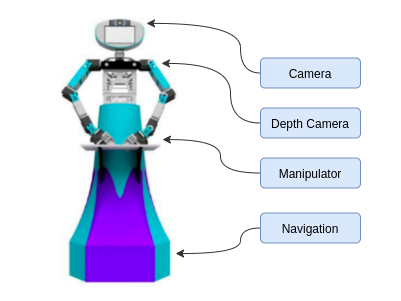
\includegraphics[scale=0.55]{images/robot-design.png}
  \caption{Diagram desain robot \emph{Dienen}.}
  \label{fig:desainrobot}
\end{figure}

Robot yang akan digunakan pada pada penelitian ini adalah robot \emph{Dienen} yang merupakan kelanjutan dari robot \emph{IRIS} \citep{dikairono2020}\citep{zanuar2019} dengan penambahan desain dari robot \emph{ICHIRO} \citep{muhtadin2019} di bagian atas robot.
Desain seperti ini secara umum dikenal sebagai desain \emph{mobile humanoid robot} \citep{mohamed2012}, yang merupakan desain gabungan antara robot \emph{mobile} dan robot \emph{humanoid}.
Seperti yang terlihat pada Gambar \ref{fig:desainrobot}, bagian bawah robot menyerupai robot \emph{mobile} dengan penggerak \emph{omnidirectional wheels} yang memungkinkan pergerakan robot secara \emph{holonomic} ke segala arah\citep{oliveira2008}, sedangkan bagian atas robot menyerupai robot \emph{humanoid} yang terdiri atas badan, kepala, dan lengan.
Dengan desain \emph{mobile humanoid robot} ini, diharapkan pengguna bisa merasakan interaksi sosial yang lebih baik dengan robot karena memiliki bentuk mendekati manusia \citep{rossi2018} sekaligus mempermudah navigasi dari robot ke berbagai tempat.

Robot \emph{Dienen} dilengkapi dengan beberapa sensor seperti IMU (\emph{inertial measurement unit}) untuk mengetahui orientasi dari robot, \emph{rotary encoder} untuk melakukan perhitungan odometri dari robot, \emph{distance sensor} untuk mendeteksi adanya objek lain di sekitar robot, sensor kamera di kepala untuk menangkap citra, dan sensor \emph{depth camera} yang nantinya bisa digunakan untuk melakukan pemetaan dari ruangan.
Selain itu robot ini juga dilengkapi dengan dua lengan seperti robot \emph{manipulator} yang bisa diatur pada berbagai posisi dan orientasi \citep{iqbal2012}.
Dengan adanya sensor dan aktuator ini diharapkan robot mampu melakukan tindakan \emph{assistive} secara sosial sesuai dengan data yang didapatkan dari sensor yang ada.
